%%%%%%%%%%%%%%%%%%%%%%%% INICIO QUADRO 01 %%%%%%%%%%%%%%%%%%%%%%%%%%%%%%%
\begin{table}[!ht]
  \centering
  \renewcommand{\tablename}{Quadro}
  \caption{}
  \label{Quadro_01}
  \begin{tabular}[t]{|ll|l|l|}
    \hline

    %%% PRÓXIMA LINHA
    \multicolumn{2}{|l|}{ \letraquadrada{A} }    &    \letraquadrada{B}    &    \letraquadrada{C}


    %%% PRÓXIMA LINHA
    \\
    \quadtitulo
    &
    \quadtitulo
    &
    \quadtitulo{Compasso}
    &
    \quadtitulo{Fórmula de compasso}

    %%% PRÓXIMA LINHA
    \\
    \begin[fragment]{lilypond}
      \transpose c c {
        \keepWithTag #'cv
        \include "nota-01.ly"
      }
    \end{lilypond}
    &
    \begin[fragment]{lilypond}
      \transpose c c { 
        \keepWithTag #'cv
        \include "nota-02.ly" 
      }
    \end{lilypond}
    &
    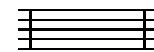
\includegraphics[scale=1]{compasso-vazio}
    &
    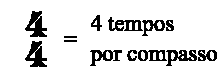
\includegraphics[scale=1]{formula-4tempos-por-compasso}


    %%% PRÓXIMA LINHA
    \\
    \hline
    \letraquadrada{D}  & \em  & \letraquadrada{E} & \letraquadrada{F}

    %%% PRÓXIMA LINHA
    \\
    \quadtitulo{Barra de Compasso}
    &
    \em
    &
    \quadtitulo{Barra Final}
    &
    \quadtitulo{Sinal de Repetição}

    %%% PRÓXIMA LINHA
    \\
    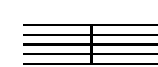
\includegraphics[scale=1]{barra-compasso}
    &
    \em
    &
    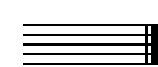
\includegraphics[scale=1]{barra-final}
    &
    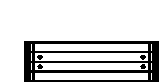
\includegraphics[scale=1]{sinal-repeticao}


    %%% PRÓXIMA LINHA
    \\
    \hline
    \letraquadrada{G}  & \em  & \letraquadrada{H} & \letraquadrada{I}

    %%% PRÓXIMA LINHA
    \\
    \quadtitulo{Mínima}
    &
    \em
    &
    \quadtitulo{Semínima}
    &
    \quadtitulo{Pausa de semibreve}


    %%% PRÓXIMA LINHA
    \\
    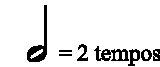
\includegraphics[scale=1]{minima}
    &
    \em
    &
    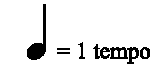
\includegraphics[scale=1]{seminima}
    &
    
\includegraphics[scale=1]{semibreve-pausa}

    %%% PRÓXIMA LINHA
    \\
    \hline
    \letraquadrada{J}  & \em  & \letraquadrada{L} & \letraquadrada{M}

    %%% PRÓXIMA LINHA
    \\
    \quadtitulo{Acordes}
    &
    \em
    &
    \quadtitulo{Técnica}
    &
    \quadtitulo{Da Capo al Fine}

    %%% PRÓXIMA LINHA
    \\
    \begin[fragment]{lilypond}
      \transpose c c { 
        \keepWithTag #'cv
        \include "acorde-Em.ly" 
      }
    \end{lilypond}

    &
    \begin[fragment]{lilypond}
      \transpose c c { 
        \keepWithTag #'cv
        \include "acorde-Am.ly" 
      }
    \end{lilypond}

    &
    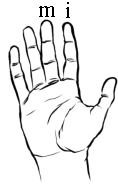
\includegraphics[scale=0.7]{mao-i-m}
    &
    \textit{D.C. al Fine}


    %%% FINAL DAS LINHAS
  \\
  \hline
  \end{tabular}
\end{table}    


%%%%%%%%%%%%%%%%%%%%%%%% FINAL QUADRO 01 %%%%%%%%%%%%%%%%%%%%%%%%%%%%%%%%




%%%%%%%%%%%%%%%%%%%%%%%% INICIO QUADRO 02 %%%%%%%%%%%%%%%%%%%%%%%%%%%%%%%
\begin{table}[!ht]
  \centering
  \renewcommand{\tablename}{Quadro}
  \caption{}
  \label{Quadro_02}
  \begin{tabular}[t]{|ll|l|}
    \hline

    %%% PRÓXIMA LINHA
    \letraquadrada{A}   &   \em    &    \letraquadrada{B}


    %%% PRÓXIMA LINHA
    \\
    \quadtitulo
    &
    \quadtitulo
    &
    \quadtitulo{Pausa de Mínima}

    %%% PRÓXIMA LINHA
    \\
    \begin[fragment]{lilypond}
      \transpose c c {
        \keepWithTag #'cv
        \include "nota-03.ly"
      }
    \end{lilypond}
    &
    \begin[fragment]{lilypond}
      \transpose c c { 
        \keepWithTag #'cv
        \include "nota-04.ly" 
      }
    \end{lilypond}
    &
    
\includegraphics[scale=1]{minima-pausa}


    %%% PRÓXIMA LINHA
    \\
    \hline
    \letraquadrada{C}  & \em  & \letraquadrada{D}

    %%% PRÓXIMA LINHA
    \\
    \quadtitulo{Acorde}
    &
    \em
    &
    \quadtitulo{Pausa de Semínima}


    %%% PRÓXIMA LINHA
    \\
    \begin[fragment]{lilypond}
      \transpose c c { 
        \keepWithTag #'cv
        \include "acorde-G.ly" 
      }
    \end{lilypond}

    &
    \em
    &
    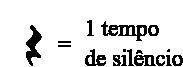
\includegraphics[scale=1]{seminima-pausa}

    %%% FINAL DAS LINHAS
  \\
  \hline
  \end{tabular}
\end{table}    


%%%%%%%%%%%%%%%%%%%%%%%% FINAL QUADRO 02 %%%%%%%%%%%%%%%%%%%%%%%%%%%%%%%%

%%%%%%%%%%%%%%%%%%%%%%%% INICIO QUADRO 03 %%%%%%%%%%%%%%%%%%%%%%%%%%%%%%%
\begin{table}[!ht]
  \centering
  \renewcommand{\tablename}{Quadro}
  \caption{}
  \label{Quadro_03}
  \begin{tabular}[t]{|l|l|l|}
    \hline

    %%% PRÓXIMA LINHA
    \letraquadrada{A}   &    \letraquadrada{B}    &   \letraquadrada{C}


    %%% PRÓXIMA LINHA
    \\
    \quadtitulo
    &
    \quadtitulo{Andamento}
    &
    \quadtitulo{Dinâmica}

    %%% PRÓXIMA LINHA
    \\
    \em
    &
    \textit{Allegro}
    &
    \textbf{\textit{f}} = forte


    %%% PRÓXIMA LINHA
    \\
    \begin[fragment]{lilypond}
      \transpose c c {
        \keepWithTag #'cv
        \include "nota-05.ly"
      }
    \end{lilypond}
    &
    \em
    &
    \textbf{\textit{p}} = piano


    %%% PRÓXIMA LINHA
    \\
    \hline
    \letraquadrada{D}  & \letraquadrada{E}  & \letraquadrada{F}

    %%% PRÓXIMA LINHA
    \\
    \quadtitulo{Acorde}
    &
    \quadtitulo{Barra Dupla}
    &
    \quadtitulo{Teoria}


    %%% PRÓXIMA LINHA
    \\
    \begin[fragment]{lilypond}
      \transpose c c { 
        \keepWithTag #'cv
        \include "acorde-C.ly" 
      }
    \end{lilypond}
    &
    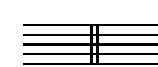
\includegraphics[scale=1]{barra-dupla}
    &
    Variação

    %%% FINAL DAS LINHAS
  \\
  \hline
  \end{tabular}
\end{table}    


%%%%%%%%%%%%%%%%%%%%%%%% FINAL QUADRO 03 %%%%%%%%%%%%%%%%%%%%%%%%%%%%%%%%


%%%%%%%%%%%%%%%%%%%%%%%% INICIO QUADRO 04 %%%%%%%%%%%%%%%%%%%%%%%%%%%%%%%
\begin{table}[!ht]
  \centering
  \renewcommand{\tablename}{Quadro}
  \caption{}
  \label{Quadro_04}
  \begin{tabular}[t]{|lll|l|}
    \hline

    %%% PRÓXIMA LINHA
    \letraquadrada{A}   &   \multicolumn{2}{|l|}{ \letraquadrada{B}}    &    \letraquadrada{C}


    %%% PRÓXIMA LINHA
    \\
     \quadtitulo
      &
      \multicolumn{2}{|l|}{\quadtitulo{Fórmula de compasso}}
      &
      \quadtitulo{Andamento}

      %%% PRÓXIMA LINHA
      \\
      \begin[fragment]{lilypond}
        \transpose c c {
          \keepWithTag #'cv
          \include "nota-06.ly"
        }
      \end{lilypond}
      &
     \multicolumn{2}{|l|}{ 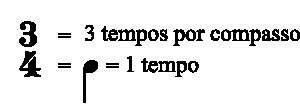
\includegraphics[scale=1]{formula-3tempos-por-compasso}}
      &
      \textit{Andante}
      \\
      \hline

      %%% PRÓXIMA LINHA
      \multicolumn{3}{|l|}{\letraquadrada{D}}  &  \letraquadrada{E}

      %%% PRÓXIMA LINHA
      \\
      \multicolumn{3}{|l|}{\quadtitulo{Acordes}}
      &
      \quadtitulo{Teoria}


      %%% PRÓXIMA LINHA
      \\
      \begin[fragment]{lilypond}
        \transpose c c { 
          \keepWithTag #'cv
          \include "acorde-G7.ly" 
        }
      \end{lilypond}

      &
      \begin[fragment]{lilypond}
        \transpose c c { 
          \keepWithTag #'cv
          \include "acorde-A7.ly" 
        }
      \end{lilypond}

      &
      \begin[fragment]{lilypond}
        \transpose c c { 
          \keepWithTag #'cv
          \include "acorde-D.ly" 
        }
      \end{lilypond}
      &
      \textit{- Harmonização
        - Transposição}


      %%% FINAL DAS LINHAS
      \\
      \hline
    \end{tabular}
  \end{table}    


%%%%%%%%%%%%%%%%%%%%%%%% FINAL QUADRO 04 %%%%%%%%%%%%%%%%%%%%%%%%%%%%%%%%


%%%%%%%%%%%%%%%%%%%%%%%% INICIO QUADRO 05 %%%%%%%%%%%%%%%%%%%%%%%%%%%%%%%
\begin{table}[!ht]
  \centering
  \renewcommand{\tablename}{Quadro}
  \caption{}
  \label{Quadro_05}
  \begin{tabular}[t]{|l|l|}
    \hline

    %%% PRÓXIMA LINHA
    \letraquadrada{A} & \letraquadrada{B}

      %%% PRÓXIMA LINHA
      \\
      \quadtitulo{Acorde}
      &
      \quadtitulo{Tonalidade - Ré menor}


      %%% PRÓXIMA LINHA
      \\
      \begin[fragment]{lilypond}
        \transpose c c { 
          \keepWithTag #'cv
          \include "acorde-Dm.ly" 
        }
      \end{lilypond}
      &
      \begin[fragment]{lilypond}
        \transpose c c {
          \keepWithTag #'cv
          \include "armadura-re-menor.ly"
        }
      \end{lilypond}



      %%% FINAL DAS LINHAS
      \\
      \hline
    \end{tabular}
  \end{table}    


%%%%%%%%%%%%%%%%%%%%%%%% FINAL QUADRO 05 %%%%%%%%%%%%%%%%%%%%%%%%%%%%%%%%



%%%%%%%%%%%%%%%%%%%%%%%% INICIO QUADRO 06 %%%%%%%%%%%%%%%%%%%%%%%%%%%%%%%
\begin{table}[!ht]
  \centering
  \renewcommand{\tablename}{Quadro}
  \caption{}
  \label{Quadro_06}
  \begin{tabular}[t]{|p{5.5cm}|l|p{2.9cm}|l|}
    \hline

    %%% PRÓXIMA LINHA
    \letraquadrada{A} & \letraquadrada{B} & \letraquadrada{C} & \letraquadrada{D}


    %%% PRÓXIMA LINHA
    \\
    \quadtitulo
    &
    \quadtitulo{Crescendo}
    &
    \quadtitulo{Decrescendo}
    &
    \quadtitulo{Ligadura de Frase}

    %%% PRÓXIMA LINHA
    \\
    \begin[fragment]{lilypond}
      \transpose c c {
        \keepWithTag #'cv
        \include "nota-07.ly"
      }
    \end{lilypond}
    &
    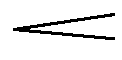
\includegraphics[scale=1]{crescendo}
    &
    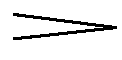
\includegraphics[scale=1]{decrescendo}
    &
    
\includegraphics[scale=1]{ligadura-frase}


    %%% PRÓXIMA LINHA
    \\
    \hline
    \letraquadrada{E} & \letraquadrada{F} & \letraquadrada{G} & \letraquadrada{H}

    %%% PRÓXIMA LINHA
    \\
    \quadtitulo{Fórmula de Compasso}
    &
    \quadtitulo{Colcheias}
    &
    \quadtitulo{Anacruse}
    &
    \quadtitulo{Escrita de Acordes}

    %%% PRÓXIMA LINHA
    \\
\begin{wrapfigure}{l}{2cm}
    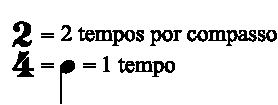
\includegraphics[scale=1]{formula-2tempos-por-compasso}
\end{wrapfigure}
    &
\begin{wrapfigure}{l}{2cm}
    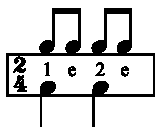
\includegraphics[scale=1]{duas-colcheias}
\end{wrapfigure}
    &
    Note que a lição \textit{``\nameref{sec:impr-em-margarida}''} na
    página \pageref{sec:impr-em-margarida} começa no 4º
    tempo do compasso.
    &
    
\includegraphics[scale=1]{escrita-acordes}

    %%% FINAL DAS LINHAS
  \\
  \hline
  \end{tabular}
\end{table}    


%%%%%%%%%%%%%%%%%%%%%%%% FINAL QUADRO 06 %%%%%%%%%%%%%%%%%%%%%%%%%%%%%%%%


%%%%%%%%%%%%%%%%%%%%%%%% INICIO QUADRO 07 %%%%%%%%%%%%%%%%%%%%%%%%%%%%%%%
\begin{table}[!ht]
  \centering
  \renewcommand{\tablename}{Quadro}
  \caption{}
  \label{Quadro_07}
  \begin{tabular}[t]{|l|l|}
    \hline

    %%% PRÓXIMA LINHA
    \letraquadrada{A} & \letraquadrada{B}


    %%% PRÓXIMA LINHA
    \\
    \quadtitulo
    &
    \quadtitulo{Mínima Pontuada}


    %%% PRÓXIMA LINHA
    \\
    \begin[fragment]{lilypond}
      \transpose c c {
        \keepWithTag #'cv
        \include "nota-08.ly"
      }
    \end{lilypond}
    &
    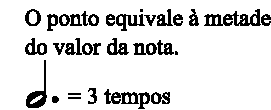
\includegraphics[scale=1]{minima-pontuada}

    %%% PRÓXIMA LINHA
    \\
    \hline
    \letraquadrada{C} & \letraquadrada{D}

    %%% PRÓXIMA LINHA
    \\
    \quadtitulo{Andamento}
    &
    \quadtitulo{Ligadura de Prolongamento}

    %%% PRÓXIMA LINHA
    \\
    \textit{Moderado}
    &
    
\includegraphics[scale=1]{ligadura-prolongamento}


    %%% FINAL DAS LINHAS
  \\
  \hline
  \end{tabular}
\end{table}    


%%%%%%%%%%%%%%%%%%%%%%%% FINAL QUADRO 07 %%%%%%%%%%%%%%%%%%%%%%%%%%%%%%%%


%%%%%%%%%%%%%%%%%%%%%%%% INICIO QUADRO 08 %%%%%%%%%%%%%%%%%%%%%%%%%%%%%%%
\begin{table}[!ht]
  \centering
  \renewcommand{\tablename}{Quadro}
  \caption{}
  \label{Quadro_08}
  \begin{tabular}[t]{|p{4cm}|l|l|}
    \hline

    %%% PRÓXIMA LINHA
    \multicolumn{2}{|l|}{ \letraquadrada{A} } & \letraquadrada{B}


    %%% PRÓXIMA LINHA
    \\
    \multicolumn{1}{|l}{ \quadtitulo }
    &
    \multicolumn{1}{l|}{ \quadtitulo }
    &
    \quadtitulo{Dinâmica}


    %%% PRÓXIMA LINHA
    \\
    \multicolumn{1}{|l}{
      \begin[fragment]{lilypond}
        \transpose c c {
          \keepWithTag #'cv
          \include "nota-09.ly"
        }
      \end{lilypond}
    }
    &
    \multicolumn{1}{l|}{
      \begin[fragment]{lilypond}
        \transpose c c {
          \keepWithTag #'cv
          \include "nota-10.ly"
        }
      \end{lilypond}
    }
    &
    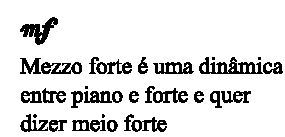
\includegraphics[scale=1]{mezzo-forte}

    %%% PRÓXIMA LINHA
    \\
    \hline
    \letraquadrada{C} & \letraquadrada{D} & \letraquadrada{E}

    %%% PRÓXIMA LINHA
    \\
    \quadtitulo{Anacruse}
    &
    \quadtitulo{Acorde}
    &
    \quadtitulo{Tonalidade - Sol Maior}
  
    %%% PRÓXIMA LINHA
    \\
    Note que a lição
    \textit{``\nameref{sec:variacoes-sobre-de-marre}''} na página
    \pageref{sec:variacoes-sobre-de-marre} começa com
    duas colcheias no 2º tempo do compasso.
    
    &
    \begin[fragment]{lilypond}
      \transpose c c { 
        \keepWithTag #'cv
        \include "acorde-D7.ly" 
      }
    \end{lilypond}
    
    &
    \begin[fragment]{lilypond}
      \transpose c c {
        \keepWithTag #'cv
        \include "armadura-sol.ly"
      }
    \end{lilypond}


    %%% FINAL DAS LINHAS
    \\
    \hline
    
  \end{tabular}
\end{table}    


%%%%%%%%%%%%%%%%%%%%%%%% FINAL QUADRO 08 %%%%%%%%%%%%%%%%%%%%%%%%%%%%%%%%



%%%%%%%%%%%%%%%%%%%%%%%% INICIO QUADRO 09 %%%%%%%%%%%%%%%%%%%%%%%%%%%%%%%
\begin{table}[!ht]
  \centering
  \renewcommand{\tablename}{Quadro}
  \caption{}
  \label{Quadro_09}
  \begin{tabular}[t]{|p{6cm}|l|}
    \hline

    %%% PRÓXIMA LINHA
    \letraquadrada{A} & \letraquadrada{B}


    %%% PRÓXIMA LINHA
    \\
    \quadtitulo{Ritmo}
    &
    \quadtitulo{Andamento}


    %%% PRÓXIMA LINHA
    \\
    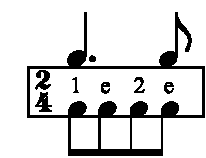
\includegraphics[scale=1]{seminima-pontuada}
    &
    \textit{Adagio}

    %%% PRÓXIMA LINHA
    \\
    \hline
    \letraquadrada{C} & \letraquadrada{D}

    %%% PRÓXIMA LINHA
    \\
    \quadtitulo{Anacruse}
    &
    \quadtitulo{Fermata}
  
    %%% PRÓXIMA LINHA
    \\
    Note que a lição \textit{``\nameref{sec:complete-melodia}''} na
    página \pageref{sec:complete-melodia} começa com
    três colcheias no 3º tempo do compasso.
    
    &
    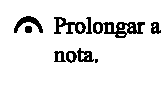
\includegraphics[scale=1]{fermata}

    %%% PRÓXIMA LINHA
    \\
    \hline
    \multicolumn{2}{|l|}{ \letraquadrada{E} }

    %%% PRÓXIMA LINHA
    \\
    \multicolumn{2}{|l|}{ \quadtitulo{Dinâmica} }
  
    %%% PRÓXIMA LINHA
    \\
    \multicolumn{2}{|l|}{ \textit{cresc.} = crescendo }
    \\
    \multicolumn{2}{|l|}{ \textit{decresc.} = diminuendo }

    %%% FINAL DAS LINHAS
    \\
    \hline
    
  \end{tabular}
\end{table}    


%%%%%%%%%%%%%%%%%%%%%%%% FINAL QUADRO 09 %%%%%%%%%%%%%%%%%%%%%%%%%%%%%%%%%


%%%%%%%%%%%%%%%%%%%%%%%% INICIO QUADRO 10 %%%%%%%%%%%%%%%%%%%%%%%%%%%%%%%
\begin{table}[!ht]
  \centering
  \renewcommand{\tablename}{Quadro}
  \caption{}
  \label{Quadro_10}
  \begin{tabular}[t]{|ll|l|}
    \hline

    %%% PRÓXIMA LINHA
    \multicolumn{2}{|l|}{ \letraquadrada{A} } & \letraquadrada{B}


    %%% PRÓXIMA LINHA
    \\
    \quadtitulo
    &
    \quadtitulo
    &
    \quadtitulo{Anacruse}


    %%% PRÓXIMA LINHA
    \\
    \multicolumn{1}{|l}{
      \begin[fragment]{lilypond}
        \transpose c c {
          \keepWithTag #'cv
          \include "nota-11.ly"
        }
      \end{lilypond}
    }
    &
    \multicolumn{1}{l|}{
      \begin[fragment]{lilypond}
        \transpose c c {
          \keepWithTag #'cv
          \include "nota-12.ly"
        }
      \end{lilypond}
    }
    &

    \multicolumn{1}{p{6.5cm}|}{ Note que a lição
      \textit{``\nameref{sec:areia}''} na página \pageref{sec:areia}
      começa com uma colcheia no 2º tempo do compasso.}

    %%% PRÓXIMA LINHA
    \\
    \hline
    \multicolumn{2}{|l|}{ \letraquadrada{C} } & \letraquadrada{D}

    %%% PRÓXIMA LINHA
    \\
    \multicolumn{2}{|l|}{ \quadtitulo{Ritmos} }
    &
    \quadtitulo{Primeira e Segunda Vez}


    %%% PRÓXIMA LINHA
    \\
    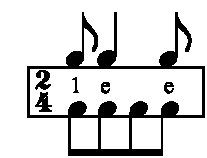
\includegraphics[scale=1]{ritmo-848}
    &
    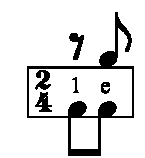
\includegraphics[scale=1]{ritmo-r8}    
    &
    \includegraphics[scale=1]


    %%% FINAL DAS LINHAS
    \\
    \hline
    
  \end{tabular}
\end{table}    


%%%%%%%%%%%%%%%%%%%%%%%% FINAL QUADRO 10 %%%%%%%%%%%%%%%%%%%%%%%%%%%%%%%%%


%%%%%%%%%%%%%%%%%%%%%%%% INICIO QUADRO 11 %%%%%%%%%%%%%%%%%%%%%%%%%%%%%%%
\begin{table}[!ht]
  \centering
  \renewcommand{\tablename}{Quadro}
  \caption{}
  \label{Quadro_11}
  \begin{tabular}[t]{|l|l|}
    \hline

    %%% PRÓXIMA LINHA
    \letraquadrada{A} & \letraquadrada{B}


    %%% PRÓXIMA LINHA
    \\
    \quadtitulo
    &
    \quadtitulo{Ritmo}


    %%% PRÓXIMA LINHA
    \\
    \begin[fragment]{lilypond}
      \transpose c c {
        \keepWithTag #'cv
        \include "nota-13.ly"
      }
    \end{lilypond}
    
    &
    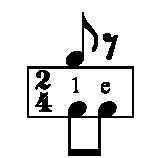
\includegraphics[scale=1]{ritmo-8r}


    %%% PRÓXIMA LINHA
    \\
    \hline
    \letraquadrada{C} & \letraquadrada{D}

    %%% PRÓXIMA LINHA
    \\
    \quadtitulo{Bequadro}
    &
    \quadtitulo{Cânone}


    %%% PRÓXIMA LINHA
    \\
    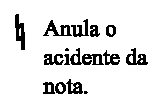
\includegraphics[scale=1]{bequadro}
    &
    \multicolumn{1}{|p{6.5cm}|}{ Gênero musical a duas ou mais vozes. A segunda voz
      deve começar a tocar quando a primeira estiver no 2. 
      Ver lição \textit{``\nameref{sec:vari-sobre-zabelinha}''}
      na página \pageref{sec:vari-sobre-zabelinha}.}
      

    %%% FINAL DAS LINHAS
    \\
    \hline
    
  \end{tabular}
\end{table}    


%%%%%%%%%%%%%%%%%%%%%%%% FINAL QUADRO 11 %%%%%%%%%%%%%%%%%%%%%%%%%%%%%%%%%


%%%%%%%%%%%%%%%%%%%%%%%% INICIO QUADRO 12 %%%%%%%%%%%%%%%%%%%%%%%%%%%%%%%
\begin{table}[!ht]
  \centering
  \renewcommand{\tablename}{Quadro}
  \caption{}
  \label{Quadro_12}
  \begin{tabular}[t]{|l|lll|}
    \hline

    %%% PRÓXIMA LINHA
    \letraquadrada{A} & \multicolumn{3}{|l|} { \letraquadrada{B} }


    %%% PRÓXIMA LINHA
    \\
    \quadtitulo
    &
    \multicolumn{3}{|l|} { \quadtitulo{Acordes} }


    %%% PRÓXIMA LINHA
    \\
    \begin[fragment]{lilypond}
      \transpose c c {
        \keepWithTag #'cv
        \include "nota-14.ly"
      }
    \end{lilypond}
    
    &
    \begin[fragment]{lilypond}
      \transpose c c { 
        \keepWithTag #'cv
        \include "acorde-A.ly" 
      }
    \end{lilypond}

    &
    \begin[fragment]{lilypond}
      \transpose c c { 
        \keepWithTag #'cv
        \include "acorde-E7.ly" 
      }
    \end{lilypond}

    &
    \begin[fragment]{lilypond}
      \transpose c c { 
        \keepWithTag #'cv
        \include "acorde-F.ly" 
      }
    \end{lilypond}


    %%% FINAL DAS LINHAS
    \\
    \hline
    
  \end{tabular}
\end{table}    


%%%%%%%%%%%%%%%%%%%%%%%% FINAL QUADRO 12 %%%%%%%%%%%%%%%%%%%%%%%%%%%%%%%%%


%%%%%%%%%%%%%%%%%%%%%%%% INICIO QUADRO 13 %%%%%%%%%%%%%%%%%%%%%%%%%%%%%%%
\begin{table}[!ht]
  \centering
  \renewcommand{\tablename}{Quadro}
  \caption{}
  \label{Quadro_13}
  \begin{tabular}[t]{|ll|l|l|}
    \hline

    %%% PRÓXIMA LINHA
    \multicolumn{2}{|l|} {\letraquadrada{A}} &  \letraquadrada{B} &  \letraquadrada{C} 


    %%% PRÓXIMA LINHA
    \\
    \quadtitulo
    &
    \quadtitulo
    &
    \quadtitulo{Acento}
    &
    \quadtitulo{Teoria}


    %%% PRÓXIMA LINHA
    \\
    \begin[fragment]{lilypond}
      \transpose c c {
        \keepWithTag #'cv
        \include "nota-15.ly"
      }
    \end{lilypond}
    
    &
    \begin[fragment]{lilypond}
      \transpose c c {
        \keepWithTag #'cv
        \include "nota-16.ly"
      }
    \end{lilypond}

    &
    \multicolumn{1}{|p{5cm}|}{ 
      
\includegraphics[scale=1]{acento}
      Indica que uma nota deverá ser reproduzida com maior intensidade
      que outras.
    }

    &
    \multicolumn{1}{|p{3cm}|}{Tom Maior e Tom Menor}



    %%% FINAL DAS LINHAS
    \\
    \hline
    
  \end{tabular}
\end{table}    


%%%%%%%%%%%%%%%%%%%%%%%% FINAL QUADRO 13 %%%%%%%%%%%%%%%%%%%%%%%%%%%%%%%%%


%%%%%%%%%%%%%%%%%%%%%%%% INICIO QUADRO 14 %%%%%%%%%%%%%%%%%%%%%%%%%%%%%%%
\begin{table}[!ht]
  \centering
  \renewcommand{\tablename}{Quadro}
  \caption{}
  \label{Quadro_14}
  \begin{tabular}[t]{|lll|}
    \hline

    %%% PRÓXIMA LINHA
    \multicolumn{3}{|l|} {\letraquadrada{A}}


    %%% PRÓXIMA LINHA
    \\
    \quadtitulo
    &
    \quadtitulo
    &
    \quadtitulo


    %%% PRÓXIMA LINHA
    \\
    \begin[fragment]{lilypond}
      \transpose c c {
        \keepWithTag #'cv
        \include "nota-17.ly"
      }
    \end{lilypond}
    
    &
    \begin[fragment]{lilypond}
      \transpose c c {
        \keepWithTag #'cv
        \include "nota-18.ly"
      }
    \end{lilypond}
    
    &
    \begin[fragment]{lilypond}
      \transpose c c {
        \keepWithTag #'cv
        \include "nota-19.ly"
      }
    \end{lilypond}

    \\
    \hline
  \end{tabular}

  \begin{tabular}[t]{|llll|}

    %%% PRÓXIMA LINHA
    \multicolumn{4}{|l|} {\letraquadrada{B}}

    %%% PRÓXIMA LINHA
    \\
    \multicolumn{4}{|l|} {\quadtitulo{Acordes}}

    %%% PRÓXIMA LINHA
    \\
    \begin[fragment]{lilypond}
      \transpose c c { 
        \keepWithTag #'cv
        \include "acorde-Bm.ly" 
      }
    \end{lilypond}

    &
    \begin[fragment]{lilypond}
      \transpose c c { 
        \keepWithTag #'cv
        \include "acorde-E.ly" 
      }
    \end{lilypond}

    &
    \begin[fragment]{lilypond}
      \transpose c c { 
        \keepWithTag #'cv
        \include "acorde-B7.ly" 
      }
    \end{lilypond}

    &
    \begin[fragment]{lilypond}
      \transpose c c { 
        \keepWithTag #'cv
        \include "acorde-Fism.ly" 
      }
    \end{lilypond}


    %%% FINAL DAS LINHAS
    \\
    \hline
    
  \end{tabular}
\end{table}    


%%%%%%%%%%%%%%%%%%%%%%%% FINAL QUADRO 14 %%%%%%%%%%%%%%%%%%%%%%%%%%%%%%%%%


%%%%%%%%%%%%%%%%%%%%%%%% INICIO QUADRO 15 %%%%%%%%%%%%%%%%%%%%%%%%%%%%%%%
\begin{table}[!ht]
  \centering
  \renewcommand{\tablename}{Quadro}
  \caption{}
  \label{Quadro_15}
  \begin{tabular}[t]{|ll|l|}
    \hline

    %%% PRÓXIMA LINHA
    \multicolumn{2}{|l|} {\letraquadrada{A}} & \letraquadrada{B}


    %%% PRÓXIMA LINHA
    \\
    \quadtitulo
    &
    \quadtitulo
    &
    \quadtitulo{Teoria}


    %%% PRÓXIMA LINHA
    \\
    \begin[fragment]{lilypond}
      \transpose c c {
        \keepWithTag #'cv
        \include "nota-20.ly"
      }
    \end{lilypond}
    
    &
    \begin[fragment]{lilypond}
      \transpose c c {
        \keepWithTag #'cv
        \include "nota-21.ly"
      }
    \end{lilypond}
    
    &
    \textit{Divisi}

    \\
    \hline
  \end{tabular}

  \begin{tabular}[t]{|llll|}

    %%% PRÓXIMA LINHA
    \multicolumn{4}{|l|} {\letraquadrada{C}}

    %%% PRÓXIMA LINHA
    \\
    \multicolumn{4}{|l|} {\quadtitulo{Acordes}}

    %%% PRÓXIMA LINHA
    \\
    \begin[fragment]{lilypond}
      \transpose c c { 
        \keepWithTag #'cv
        \include "acorde-C7.ly" 
      }
    \end{lilypond}

    &
    \begin[fragment]{lilypond}
      \transpose c c { 
        \keepWithTag #'cv
        \include "acorde-Gm.ly" 
      }
    \end{lilypond}

    &
    \begin[fragment]{lilypond}
      \transpose c c { 
        \keepWithTag #'cv
        \include "acorde-Cm.ly" 
      }
    \end{lilypond}

    &
    \begin[fragment]{lilypond}
      \transpose c c { 
        \keepWithTag #'cv
        \include "acorde-Bb.ly" 
      }
    \end{lilypond}


    %%% FINAL DAS LINHAS
    \\
    \hline
    
  \end{tabular}
\end{table}    


%%%%%%%%%%%%%%%%%%%%%%%% FINAL QUADRO 15 %%%%%%%%%%%%%%%%%%%%%%%%%%%%%%%%%


%%%%%%%%%%%%%%%%%%%%%%%% INICIO QUADRO 16 %%%%%%%%%%%%%%%%%%%%%%%%%%%%%%%
\begin{table}[!ht]
  \centering
  \renewcommand{\tablename}{Quadro}
  \caption{}
  \label{Quadro_16}
  \begin{tabular}[t]{|ll|}
    \hline

    %%% PRÓXIMA LINHA
    \multicolumn{2}{|l|} {\letraquadrada{A}}


    %%% PRÓXIMA LINHA
    \\
    \quadtitulo
    &
    \quadtitulo


    %%% PRÓXIMA LINHA
    \\
    \begin[fragment]{lilypond}
      \transpose c c {
        \keepWithTag #'cv
        \include "nota-22.ly"
      }
    \end{lilypond}
    
    &
    \begin[fragment]{lilypond}
      \transpose c c {
        \keepWithTag #'cv
        \include "nota-23.ly"
      }
    \end{lilypond}
    
    \\
    \hline
  \end{tabular}
\end{table}    


%%%%%%%%%%%%%%%%%%%%%%%% FINAL QUADRO 16 %%%%%%%%%%%%%%%%%%%%%%%%%%%%%%%%%




